% Editable native annotations around unchanged verified IDE photographs.
\par
\begin{figure}[htbp]
\centering
\newsavebox{\MARSdeltascancandidateBox}
\sbox{\MARSdeltascancandidateBox}{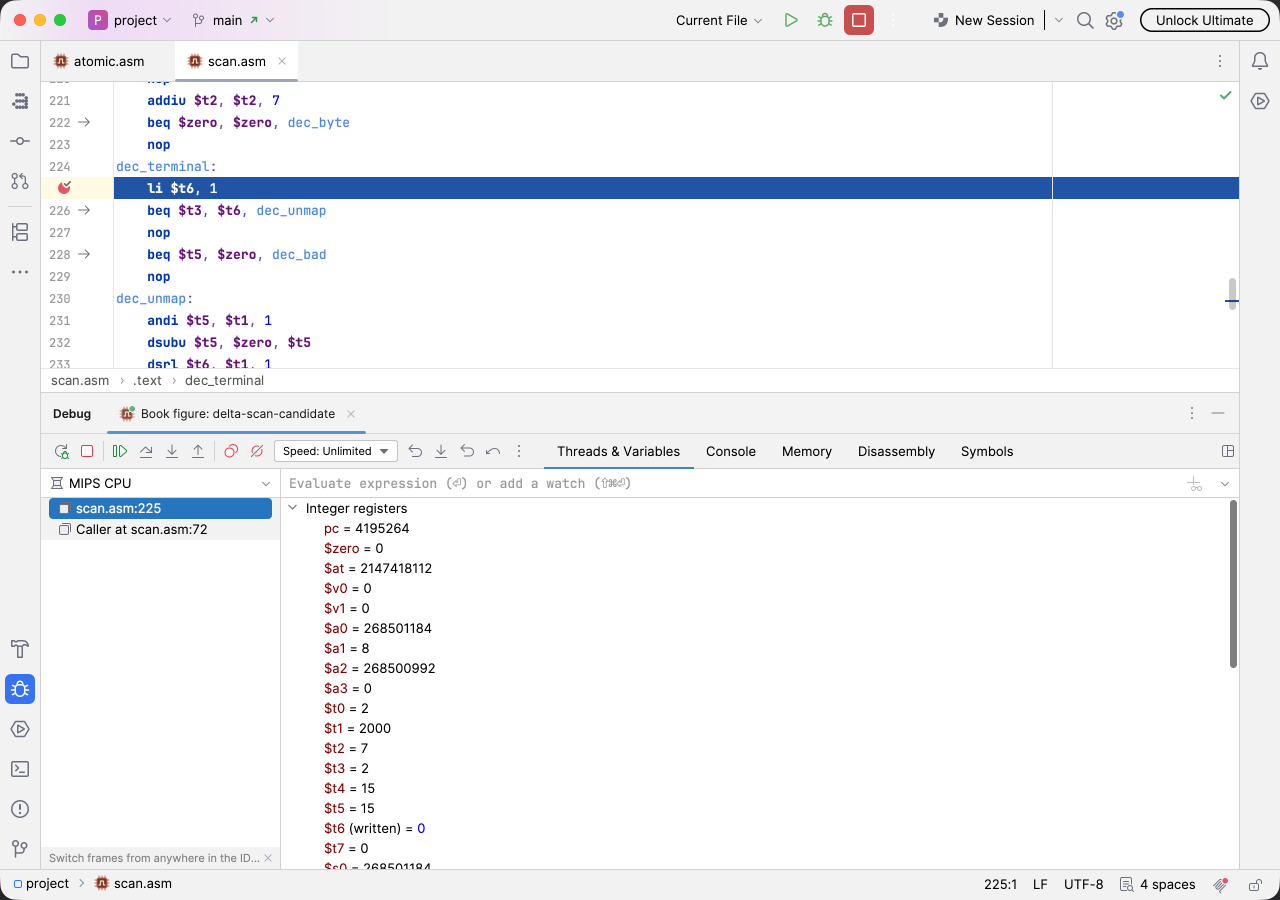
\includegraphics[artifact]{packages/023-delta-varint/captures/f02/candidate.png}}
\newsavebox{\MARSdeltascancommittedBox}
\sbox{\MARSdeltascancommittedBox}{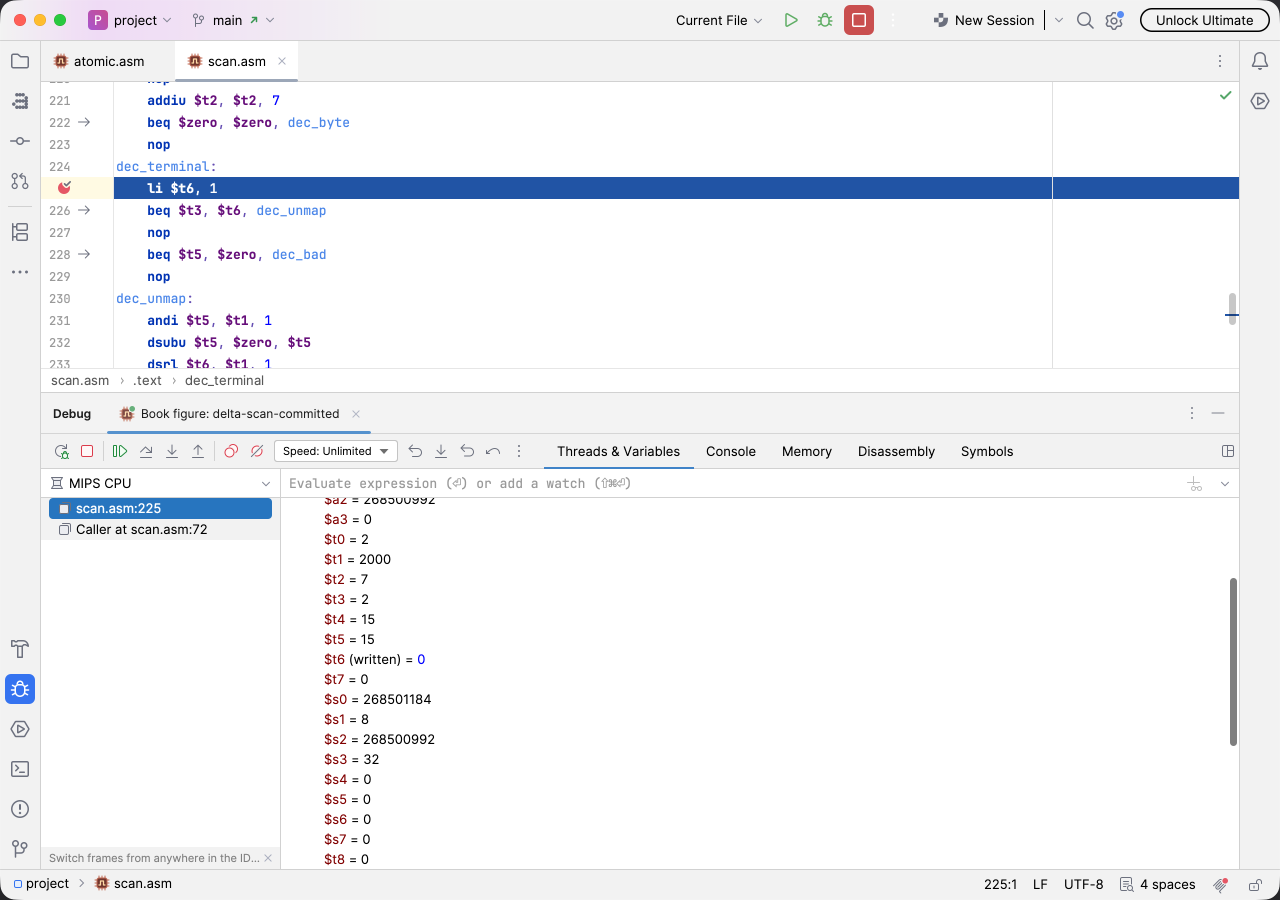
\includegraphics[artifact]{packages/023-delta-varint/captures/f02/committed.png}}
\newsavebox{\MARSdeltascanstreamBox}
\sbox{\MARSdeltascanstreamBox}{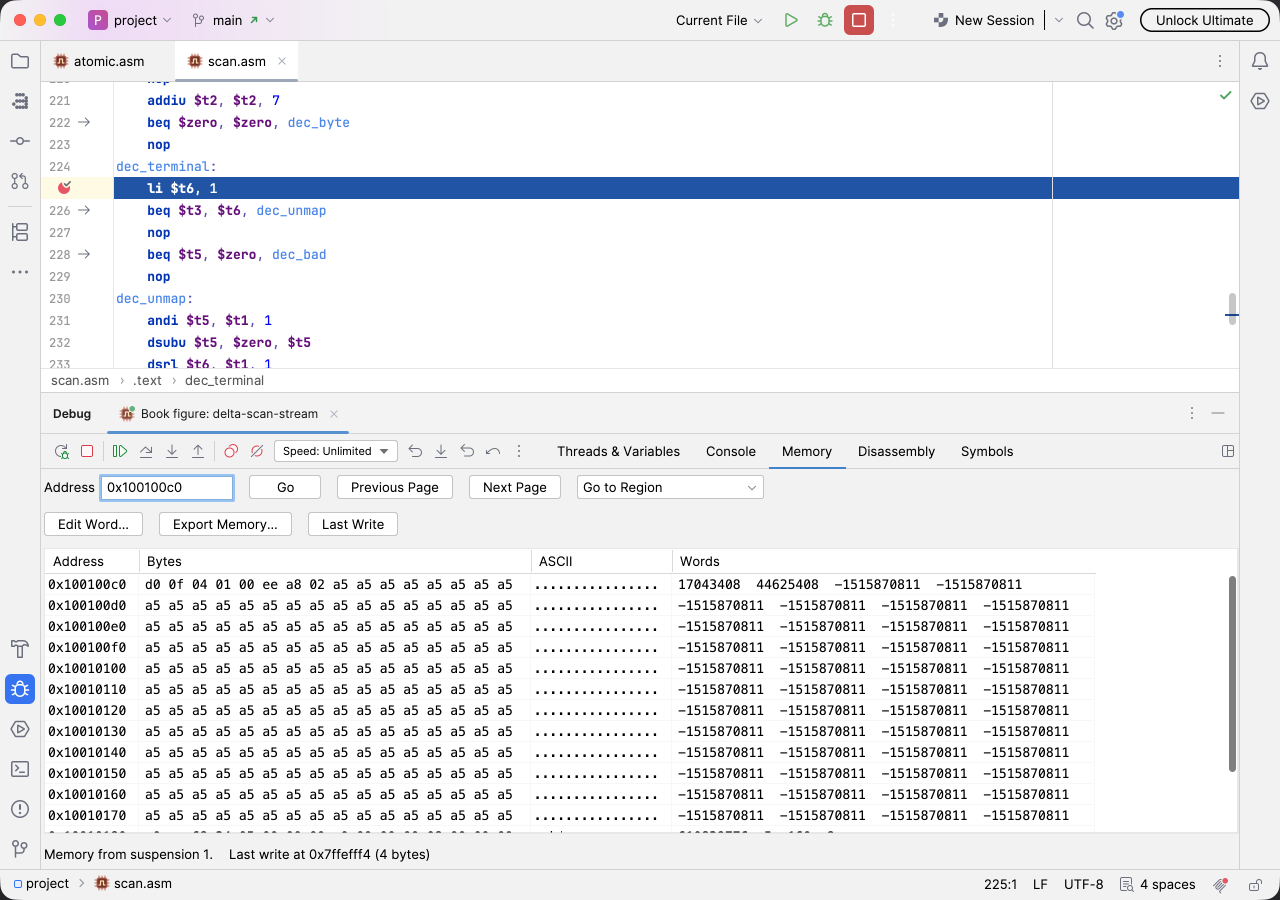
\includegraphics[artifact]{packages/023-delta-varint/captures/f02/stream.png}}
\newsavebox{\MARSdeltascanwordsBox}
\sbox{\MARSdeltascanwordsBox}{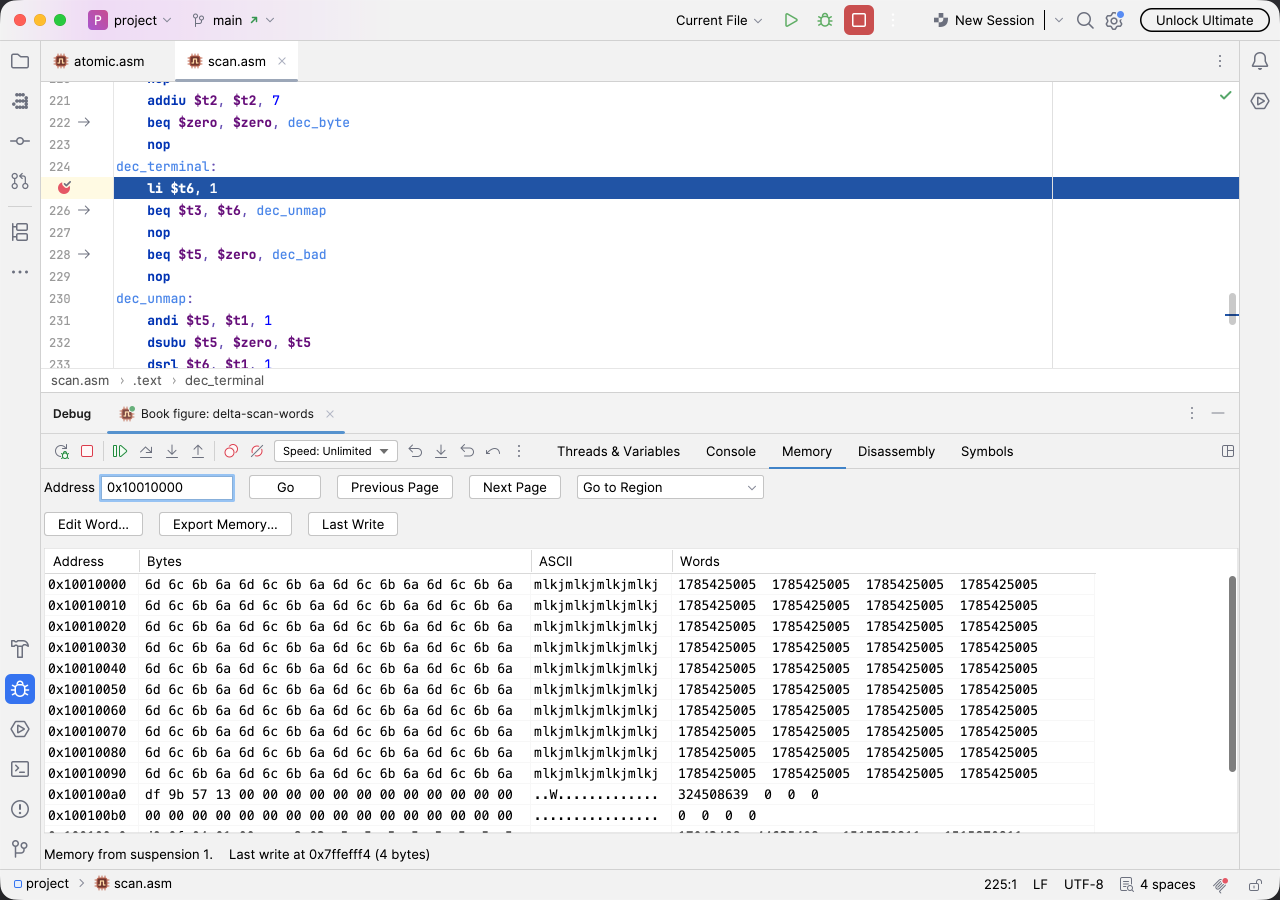
\includegraphics[artifact]{packages/023-delta-varint/captures/f02/words.png}}
\newsavebox{\MARSdeltascancontrolBox}
\sbox{\MARSdeltascancontrolBox}{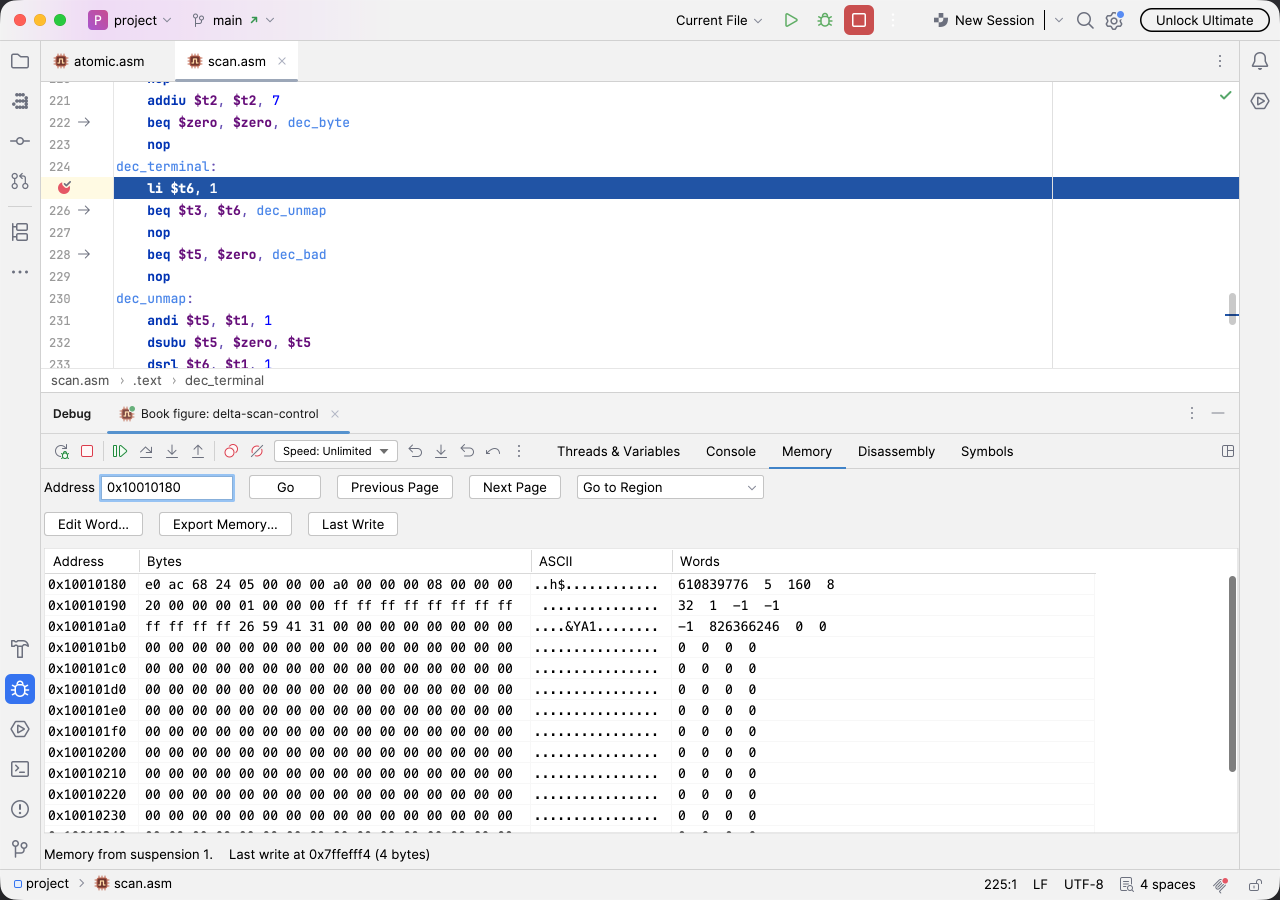
\includegraphics[artifact]{packages/023-delta-varint/captures/f02/control.png}}
\edef\MARSdeltascansourceLeft{\the\dimexpr0.036718750\wd\MARSdeltascancandidateBox\relax}
\edef\MARSdeltascansourceBottom{\the\dimexpr0.774444444\ht\MARSdeltascancandidateBox\relax}
\edef\MARSdeltascansourceRight{\the\dimexpr0.713281250\wd\MARSdeltascancandidateBox\relax}
\edef\MARSdeltascansourceTop{\the\dimexpr0.170000000\ht\MARSdeltascancandidateBox\relax}
\edef\MARSdeltascancandidateLeft{\the\dimexpr0.246093750\wd\MARSdeltascancandidateBox\relax}
\edef\MARSdeltascancandidateBottom{\the\dimexpr0.178888889\ht\MARSdeltascancandidateBox\relax}
\edef\MARSdeltascancandidateRight{\the\dimexpr0.553906250\wd\MARSdeltascancandidateBox\relax}
\edef\MARSdeltascancandidateTop{\the\dimexpr0.773333333\ht\MARSdeltascancandidateBox\relax}
\edef\MARSdeltascancommittedLeft{\the\dimexpr0.246093750\wd\MARSdeltascancommittedBox\relax}
\edef\MARSdeltascancommittedBottom{\the\dimexpr0.077777778\ht\MARSdeltascancommittedBox\relax}
\edef\MARSdeltascancommittedRight{\the\dimexpr0.553906250\wd\MARSdeltascancommittedBox\relax}
\edef\MARSdeltascancommittedTop{\the\dimexpr0.874444444\ht\MARSdeltascancommittedBox\relax}
\edef\MARSdeltascanstreamLeft{\the\dimexpr0.034375000\wd\MARSdeltascanstreamBox\relax}
\edef\MARSdeltascanstreamBottom{\the\dimexpr0.334444444\ht\MARSdeltascanstreamBox\relax}
\edef\MARSdeltascanstreamRight{\the\dimexpr0.584375000\wd\MARSdeltascanstreamBox\relax}
\edef\MARSdeltascanstreamTop{\the\dimexpr0.608888889\ht\MARSdeltascanstreamBox\relax}
\edef\MARSdeltascanwordsLeft{\the\dimexpr0.034375000\wd\MARSdeltascanwordsBox\relax}
\edef\MARSdeltascanwordsBottom{\the\dimexpr0.311111111\ht\MARSdeltascanwordsBox\relax}
\edef\MARSdeltascanwordsRight{\the\dimexpr0.584375000\wd\MARSdeltascanwordsBox\relax}
\edef\MARSdeltascanwordsTop{\the\dimexpr0.608888889\ht\MARSdeltascanwordsBox\relax}
\edef\MARSdeltascancontrolLeft{\the\dimexpr0.034375000\wd\MARSdeltascancontrolBox\relax}
\edef\MARSdeltascancontrolBottom{\the\dimexpr0.311111111\ht\MARSdeltascancontrolBox\relax}
\edef\MARSdeltascancontrolRight{\the\dimexpr0.584375000\wd\MARSdeltascancontrolBox\relax}
\edef\MARSdeltascancontrolTop{\the\dimexpr0.608888889\ht\MARSdeltascancontrolBox\relax}
\begin{tikzpicture}[alt={Six annotated details at dec_terminal show scan t0 equal two and unsigned candidate t1 equal 2000. Working committed counts s5 and s6 are zero. Input begins d0 0f, and the output arena retains its sentinel words. The first candidate has not yet passed canonicality, inverse mapping or reconstructed-range checks.}]
\node[anchor=north west,inner sep=0,font=\small\bfseries] (source-title) at (6mm,0) {Next instruction at this boundary};
\node[anchor=north west,inner sep=0] (source) at ([yshift=-1mm]source-title.south west) {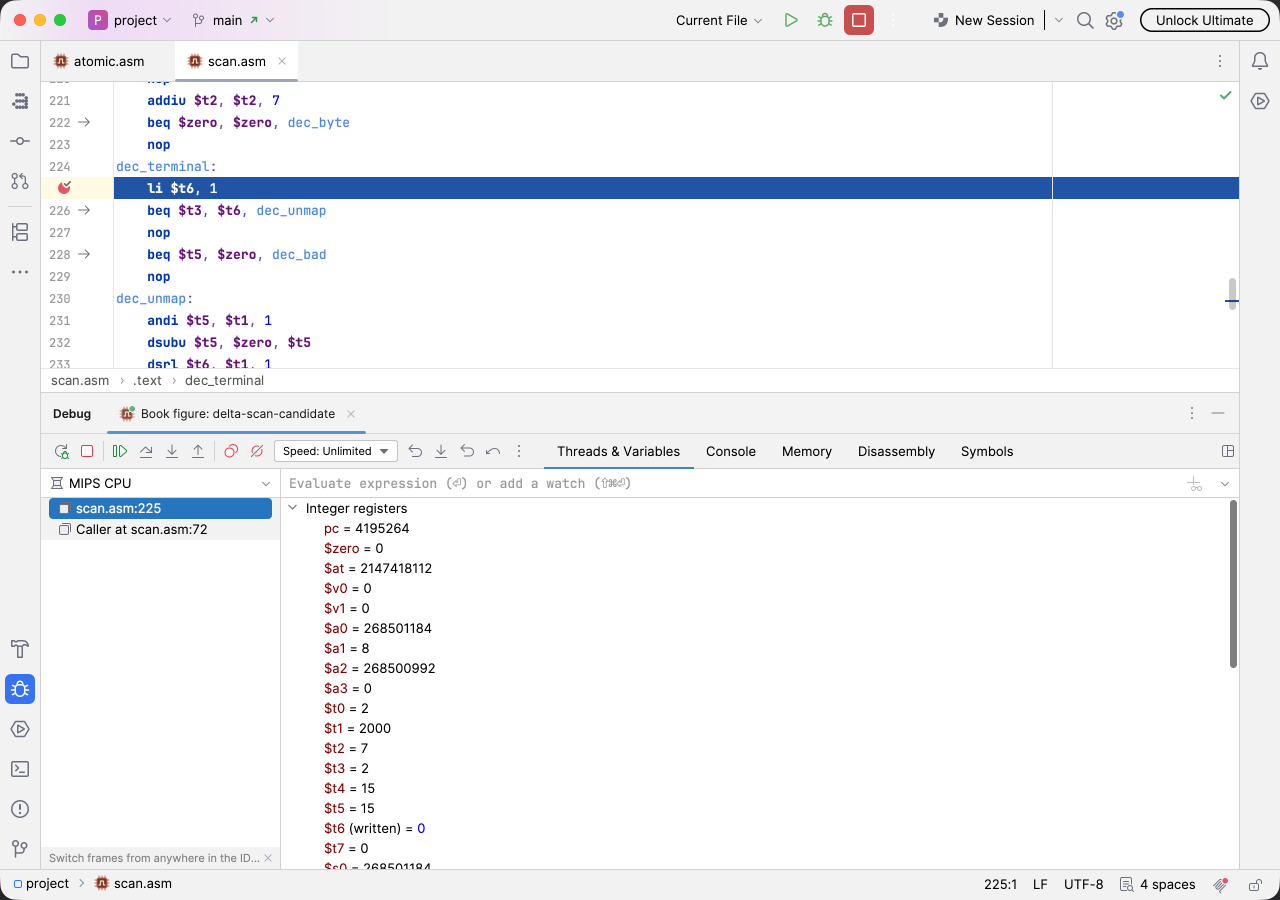
\includegraphics[width=0.54\linewidth,artifact,trim={\MARSdeltascansourceLeft{} \MARSdeltascansourceBottom{} \MARSdeltascansourceRight{} \MARSdeltascansourceTop{}},clip]{packages/023-delta-varint/captures/f02/candidate.png}};
\begin{scope}[shift={(source.south west)},x={($(source.south east)-(source.south west)$)},y={($(source.north west)-(source.south west)$)}]
\draw[black,line width=0.7pt] (0.215625000,0.080000000) rectangle (0.531250000,0.520000000);
\node[draw=black,fill=white,circle,inner sep=1.5pt,font=\footnotesize] at ($(0.215625000,0.520000000)+(-3mm,0)$) {1};
\end{scope}
\node[anchor=north west,inner sep=0,font=\small\bfseries] (candidate-title) at (0.58\linewidth,0 |- source-title.north) {Private scan and unsigned candidate};
\node[anchor=north west,inner sep=0] (candidate) at ([yshift=-1mm]candidate-title.south west) {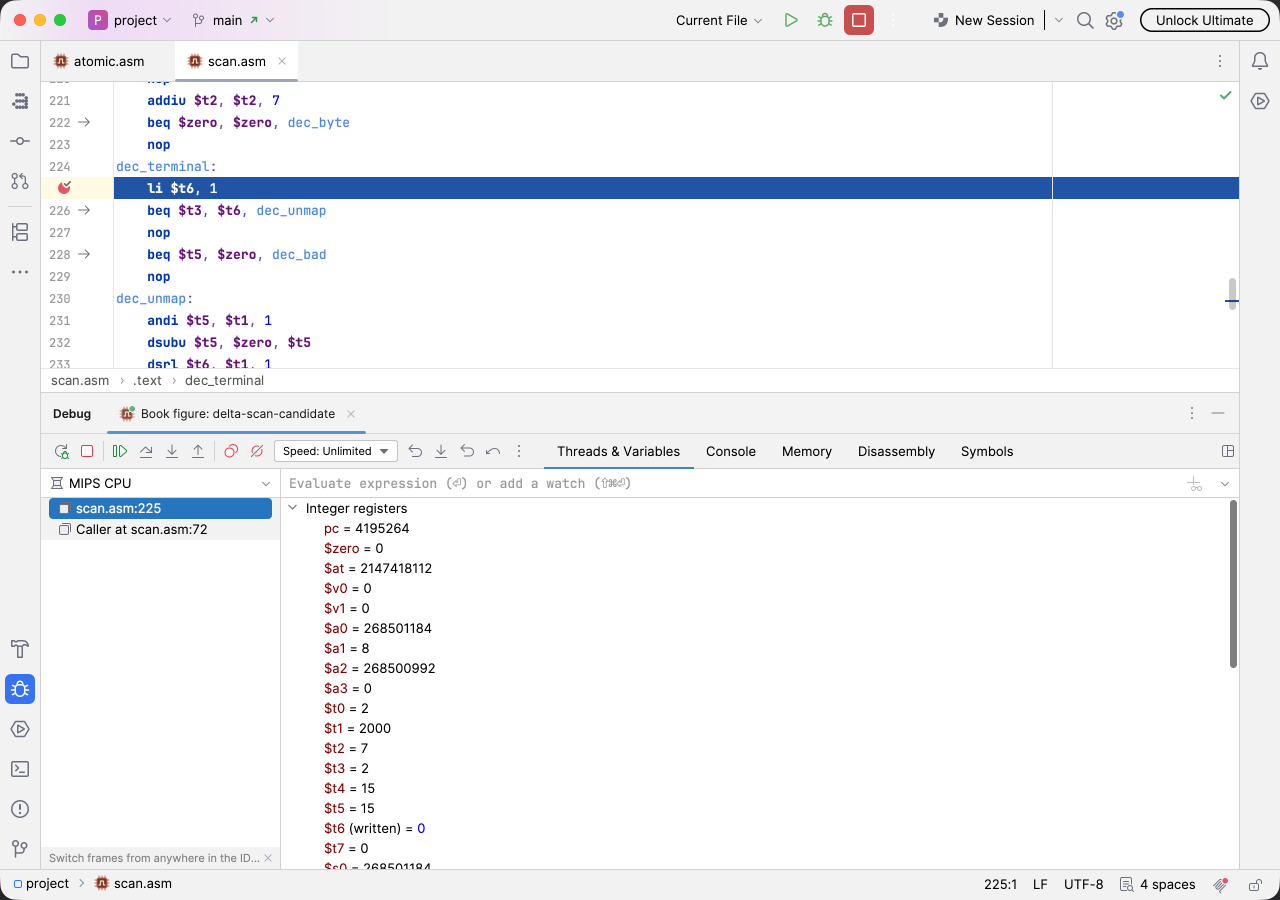
\includegraphics[width=0.42\linewidth,artifact,trim={\MARSdeltascancandidateLeft{} \MARSdeltascancandidateBottom{} \MARSdeltascancandidateRight{} \MARSdeltascancandidateTop{}},clip]{packages/023-delta-varint/captures/f02/candidate.png}};
\begin{scope}[shift={(candidate.south west)},x={($(candidate.south east)-(candidate.south west)$)},y={($(candidate.north west)-(candidate.south west)$)}]
\draw[black,line width=0.7pt] (0.023437500,0.023255814) rectangle (0.304687500,0.953488372);
\node[draw=black,fill=white,circle,inner sep=1.5pt,font=\footnotesize] at ($(0.023437500,0.953488372)+(-3mm,0)$) {2};
\end{scope}
\node[anchor=north west,inner sep=0,font=\small\bfseries] (committed-title) at ([yshift=-1mm]source.south west) {Working committed counts};
\node[anchor=north west,inner sep=0] (committed) at ([yshift=-1mm]committed-title.south west) {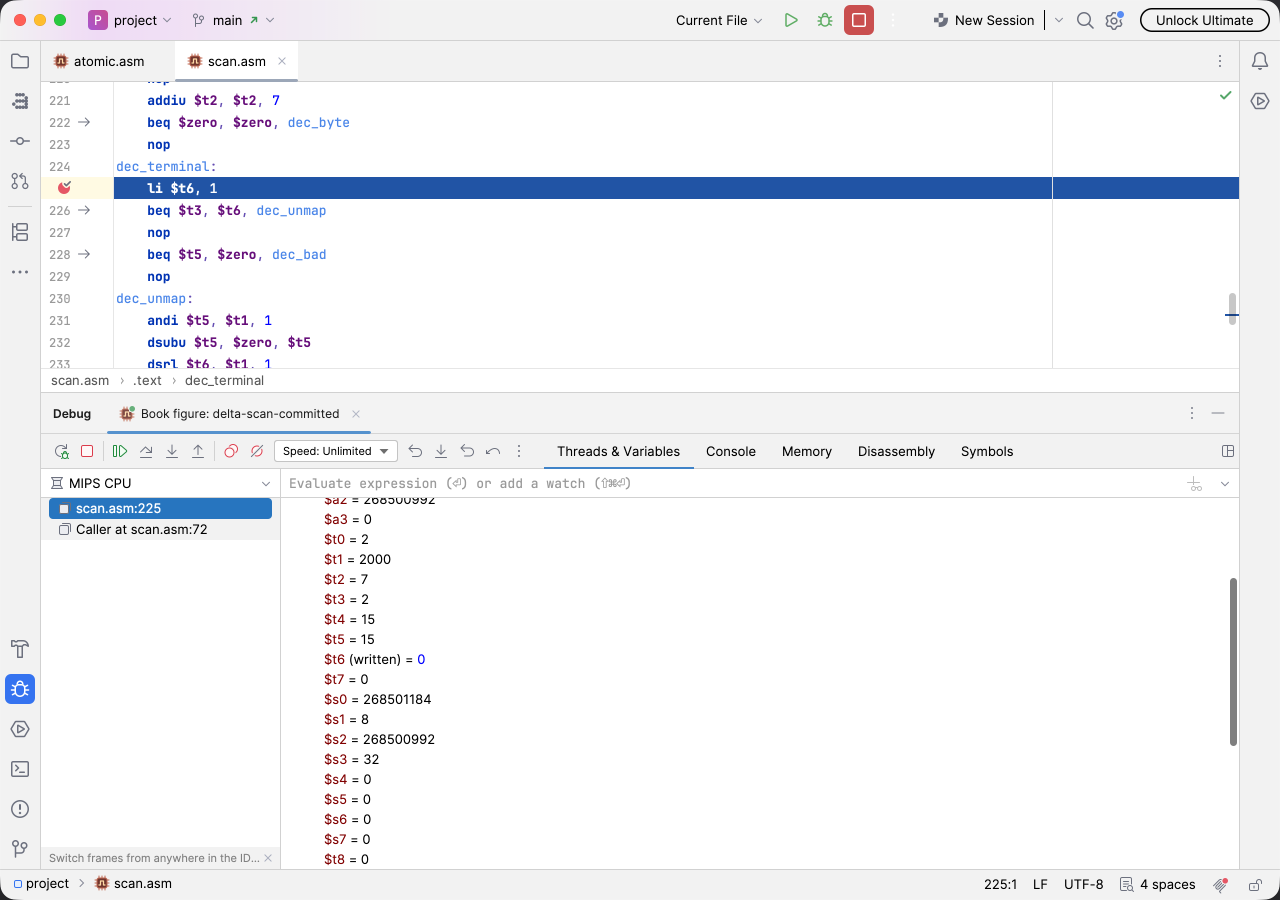
\includegraphics[width=0.42\linewidth,artifact,trim={\MARSdeltascancommittedLeft{} \MARSdeltascancommittedBottom{} \MARSdeltascancommittedRight{} \MARSdeltascancommittedTop{}},clip]{packages/023-delta-varint/captures/f02/committed.png}};
\begin{scope}[shift={(committed.south west)},x={($(committed.south east)-(committed.south west)$)},y={($(committed.north west)-(committed.south west)$)}]
\draw[black,line width=0.7pt] (0.023437500,0.023255814) rectangle (0.226562500,0.953488372);
\node[draw=black,fill=white,circle,inner sep=1.5pt,font=\footnotesize] at ($(0.023437500,0.953488372)+(-3mm,0)$) {3};
\end{scope}
\node[anchor=north west,inner sep=0,font=\small\bfseries] (stream-title) at ([yshift=-1mm]committed.south west) {Input stream bytes};
\node[anchor=north west,inner sep=0] (stream) at ([yshift=-1mm]stream-title.south west) {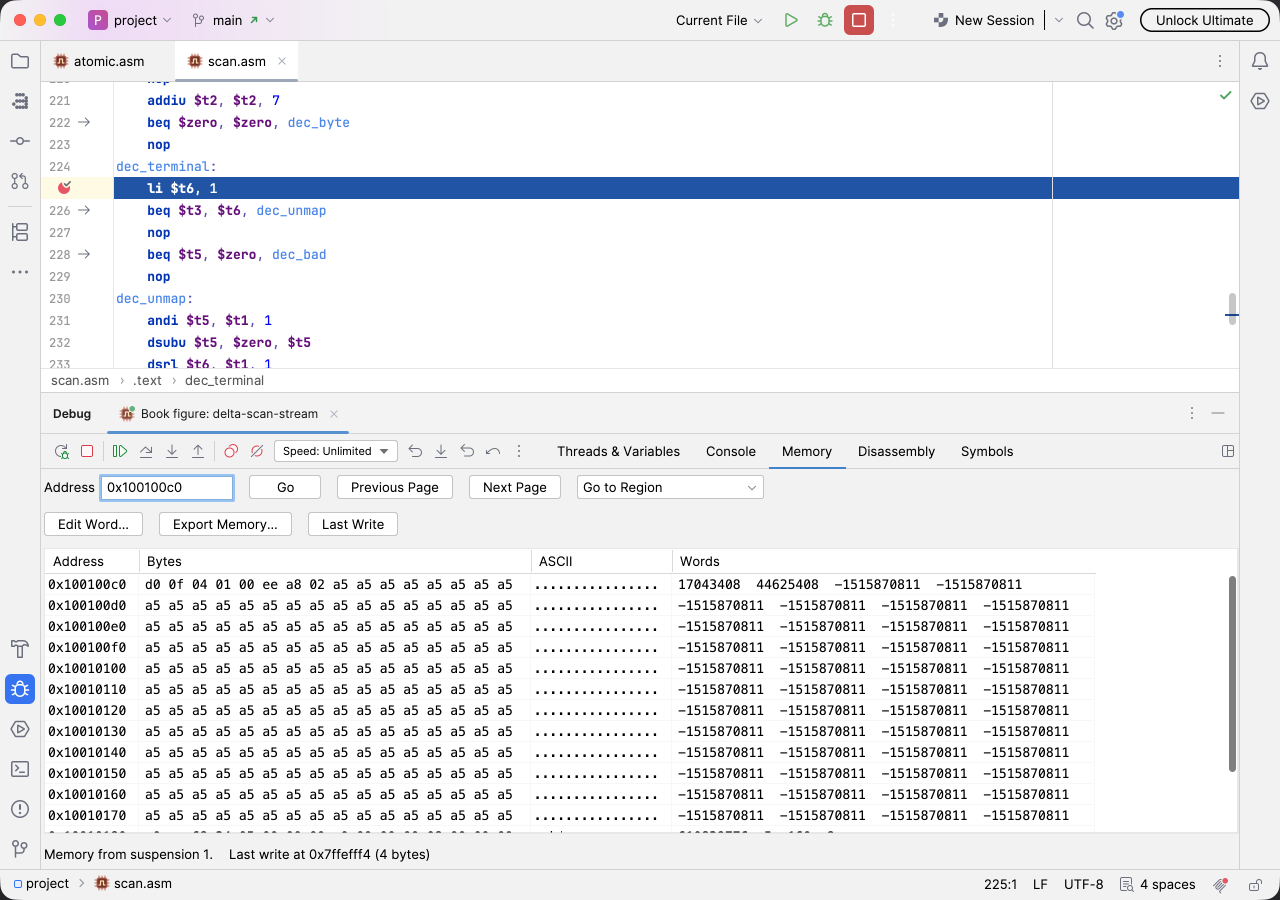
\includegraphics[width=0.84\linewidth,artifact,trim={\MARSdeltascanstreamLeft{} \MARSdeltascanstreamBottom{} \MARSdeltascanstreamRight{} \MARSdeltascanstreamTop{}},clip]{packages/023-delta-varint/captures/f02/stream.png}};
\begin{scope}[shift={(stream.south west)},x={($(stream.south east)-(stream.south west)$)},y={($(stream.north west)-(stream.south west)$)}]
\draw[black,line width=0.7pt] (0.194672131,0.078431373) rectangle (0.997950820,0.490196078);
\node[draw=black,fill=white,circle,inner sep=1.5pt,font=\footnotesize] at ($(0,0.490196078)+(-3mm,0)$) {4};
\end{scope}
\node[anchor=north west,inner sep=0,font=\small\bfseries] (words-title) at ([yshift=-1mm]stream.south west) {Output words before commitment};
\node[anchor=north west,inner sep=0] (words) at ([yshift=-1mm]words-title.south west) {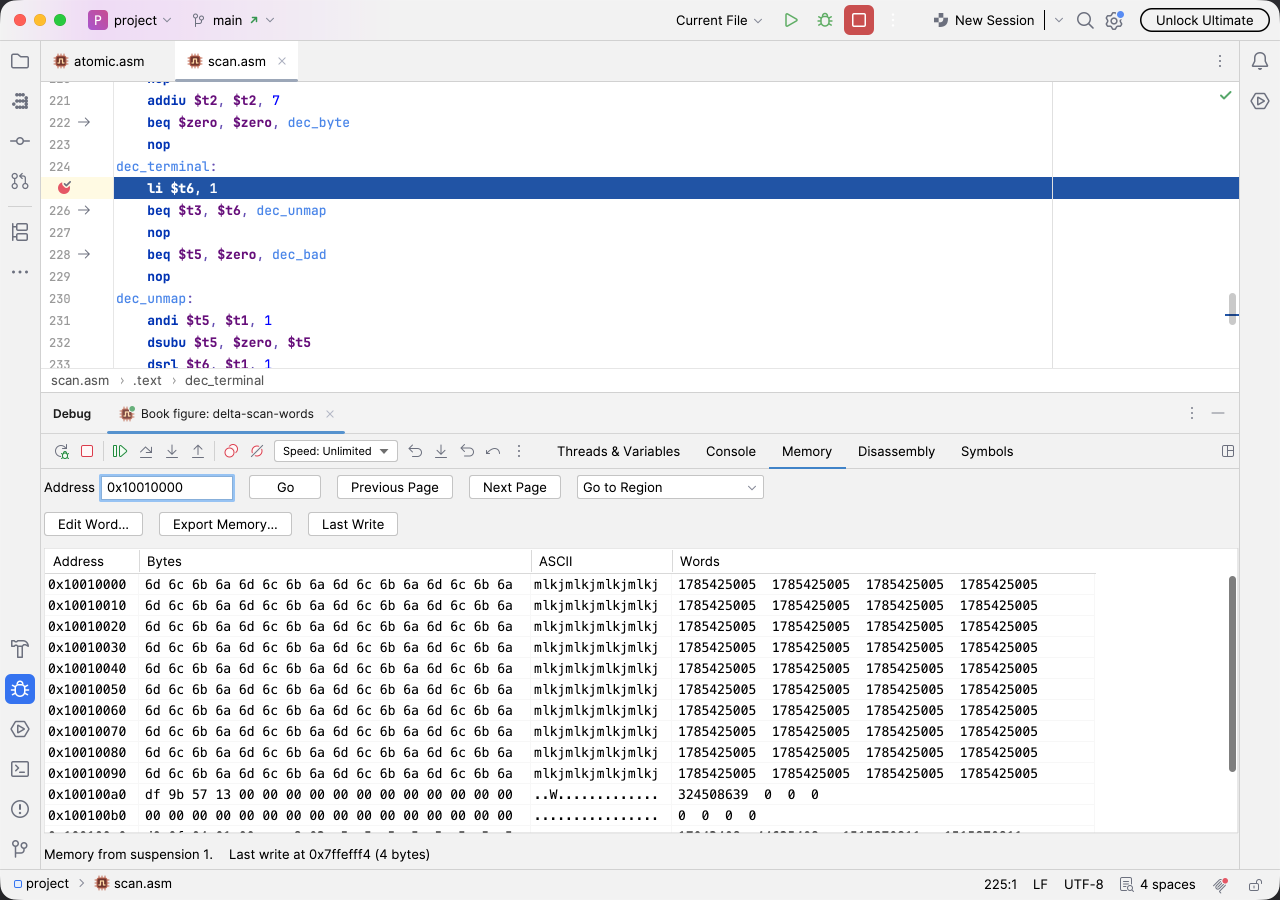
\includegraphics[width=0.84\linewidth,artifact,trim={\MARSdeltascanwordsLeft{} \MARSdeltascanwordsBottom{} \MARSdeltascanwordsRight{} \MARSdeltascanwordsTop{}},clip]{packages/023-delta-varint/captures/f02/words.png}};
\begin{scope}[shift={(words.south west)},x={($(words.south east)-(words.south west)$)},y={($(words.north west)-(words.south west)$)}]
\draw[black,line width=0.7pt] (0.194672131,0.055555556) rectangle (0.997950820,0.638888889);
\node[draw=black,fill=white,circle,inner sep=1.5pt,font=\footnotesize] at ($(0,0.638888889)+(-3mm,0)$) {5};
\end{scope}
\node[anchor=north west,inner sep=0,font=\small\bfseries] (control-title) at ([yshift=-1mm]words.south west) {Caller controls and saved counts};
\node[anchor=north west,inner sep=0] (control) at ([yshift=-1mm]control-title.south west) {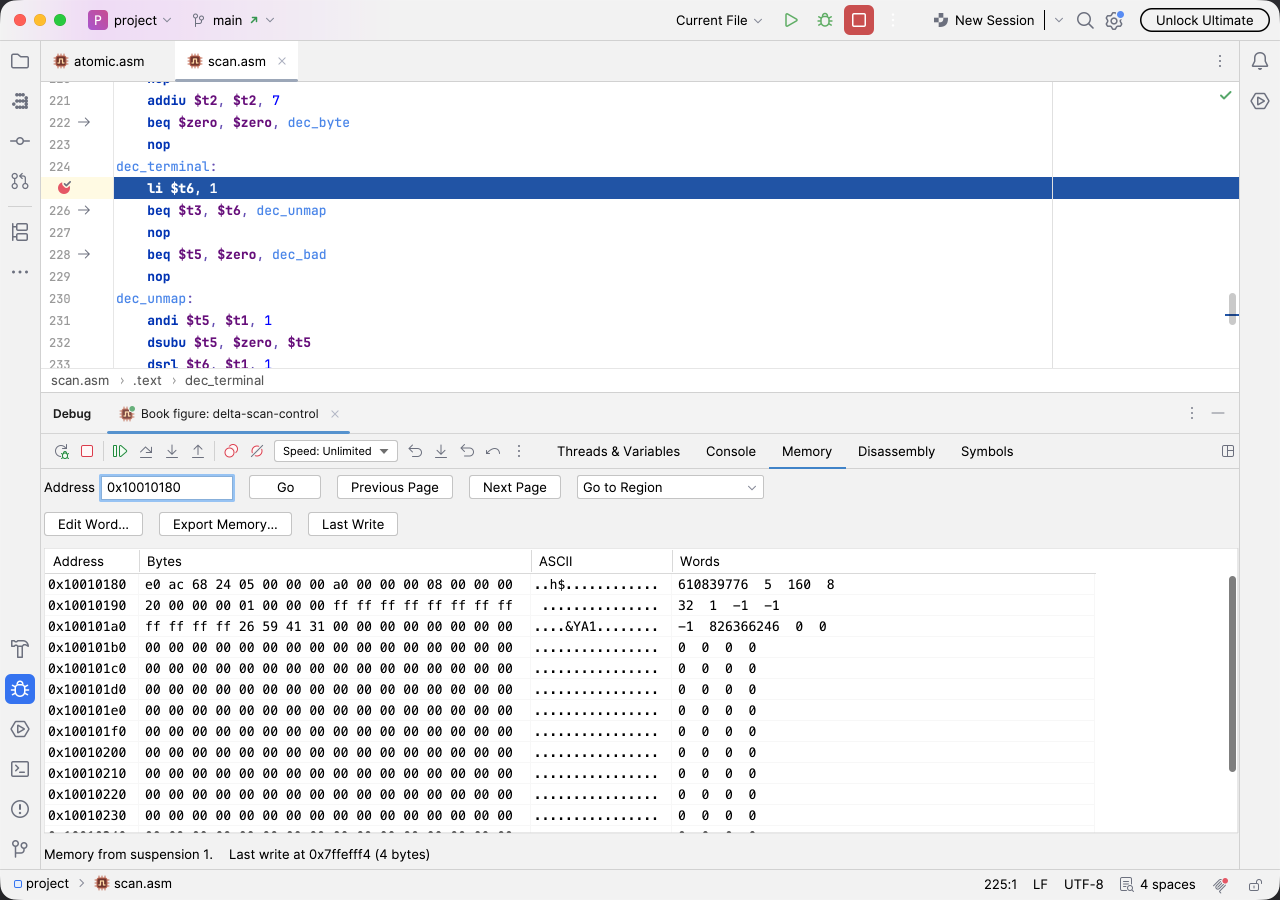
\includegraphics[width=0.84\linewidth,artifact,trim={\MARSdeltascancontrolLeft{} \MARSdeltascancontrolBottom{} \MARSdeltascancontrolRight{} \MARSdeltascancontrolTop{}},clip]{packages/023-delta-varint/captures/f02/control.png}};
\begin{scope}[shift={(control.south west)},x={($(control.south east)-(control.south west)$)},y={($(control.north west)-(control.south west)$)}]
\draw[black,line width=0.7pt] (0.194672131,0.055555556) rectangle (0.997950820,0.638888889);
\node[draw=black,fill=white,circle,inner sep=1.5pt,font=\footnotesize] at ($(0,0.638888889)+(-3mm,0)$) {6};
\end{scope}
\end{tikzpicture}
\par\smallskip
\begin{minipage}{\linewidth}
\small
\begin{enumerate}
\setlength{\itemsep}{2pt}
\setlength{\parsep}{0pt}
\item The stop is inside the decoder at \texttt{dec\_terminal}, before the terminal-group checks. This is an internal candidate boundary, rather than a completed function return.
\item \texttt{t0 = 2} is the private scan position; \texttt{t1 = 2000} is the assembled unsigned candidate. Neither is a committed return count.
\item Working counts \texttt{s5 = 0} and \texttt{s6 = 0} still mark an empty committed prefix. They will change only after validation, inverse mapping, range checking and the destination store.
\item The stream begins \texttt{d0 0f}: payloads 80 and 15 give $80+15\cdot128=2000$. Its even mapping reconstructs the first reading as 1000, provided the remaining checks pass.
\item Output words still contain the supplied \texttt{0x6a6b6c6d} sentinel, stored low byte first as \texttt{6d 6c 6b 6a}. No reading has been written at this stop.
\item The controls select eight input bytes, capacity 32 readings and method one. Saved input/output counts remain $-1$ because the caller cannot publish a result until the function returns.
\end{enumerate}
\end{minipage}
\caption{A private scan can advance before any input or output is committed.}
\label{capture:023-delta-varint-f02}
\label{delta-f02}
\end{figure}
\par
